\title{Probabilistic PCA}

\subsection{Probabilistic PCA}

Probabilistic principal components analysis (probabilistic PCA) is
useful for analyzing data via a lower dimensional latent space
\citep{tipping1999probabilistic}. It is often
used when there are missing values in the data or for multidimensional
scaling.

We'll run through a quick tutorial to implement it in Edward below.
The full script can be accessed at
\href{https://github.com/blei-lab/edward/blob/master/examples/probabilistic_pca.py}
{\texttt{examples/probabilistic_pca.py}} in the Github repository.

\subsubsection{Data}

We use simulated data. We'll talk about the individual variables and
what they stand for in the next section. For this example, each data
point is 2-dimensional, $\mathbf{x}_n\in\mathbb{R}^2$.

\begin{lstlisting}[language=Python]
def build_toy_dataset(N, D, K, sigma=1):
  x_train = np.zeros((D, N))
  w = np.random.normal(0.0, 2.0, size=(D, K))
  z = np.random.normal(0.0, 1.0, size=(K, N))
  mean = np.dot(w, z)
  for d in range(D):
    for n in range(N):
      x_train[d, n] = np.random.normal(mean[d, n], sigma)

  return x_train

N = 5000  # number of data points
D = 2  # data dimensionality
K = 1  # latent dimensionality

x_train = build_toy_dataset(N, D, K)
\end{lstlisting}

This generates a dataset that looks like this:

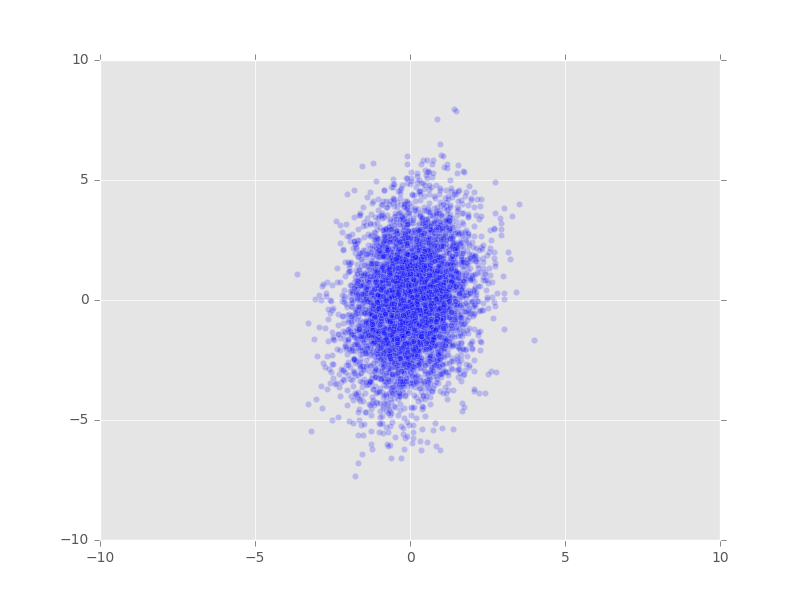
\includegraphics[width=450px]{/images/ppca-fig0.png}

\subsubsection{Model}

Consider a set of $N$ data points, $X = \{\mathbf{x}_n\}$, where each
data point is $d$-dimensional, $\mathbf{x}_n \in \mathbb{R}^D$.

While our data operates in dimension $D$, we will use latent variables
$\mathbf{z}_n \in \mathbb{R}^K$ for each data point $\mathbf{x}_n$
with lower latent dimension, $K < D$. The set of principal axes
$\mathbf{W}$ relates our latent variables to our actual data.

Thus, we have that
\begin{equation*}
\mathbf{z} \sim N(0, \mathbf{I}),
\end{equation*}
and that
\begin{equation*}
\mathbf{x} \mid \mathbf{z} \sim N(\mathbf{Wz} + \mu, \sigma^2\mathbf{I}),
\end{equation*}
where $\mathbf{\epsilon} \sim N(0, \sigma^2\mathbf{I})$.

Because of the dependence on $\mathbf{Wz}$, we don't want to solely
want to infer the original principal axes (as would be done in the
vanilla PCA model). Rather, we aim to model the principal axes with
respect to the latent variables.

For our marginal distribution, we get that
\begin{equation*}
x \sim N(0, \mathbf{W}\mathbf{W}^Y + \sigma^2\mathbf{I}).
\end{equation*}

Note here that regular PCA is simply the specific case of
Probabilistic PCA, as $\sigma^2 \to 0$.

We set up our model below, forming creating a prior distribution over
our variables of interest.

\begin{lstlisting}[language=Python]
w = Normal(mu=tf.zeros([D, K]), sigma=2.0 * tf.ones([D, K]))
z = Normal(mu=tf.zeros([N, K]), sigma=tf.ones([N, K]))
x = Normal(mu=tf.matmul(w, z, transpose_b=True), sigma=tf.ones([D, N]))

\end{lstlisting}

\subsubsection{Inference}

Since the principal axes $\mathbf{W}$ cannot be analytically
determined, we must use some inference method. Below, we set up our
inference variables and then run a chosen algorithm. For this
example, we minimize the $\text{KL}(q\|p)$ divergence measure.

\begin{lstlisting}[language=Python]
qw = Normal(mu=tf.Variable(tf.random_normal([D, K])),
            sigma=tf.nn.softplus(tf.Variable(tf.random_normal([D, K]))))
qz = Normal(mu=tf.Variable(tf.random_normal([N, K])),
            sigma=tf.nn.softplus(tf.Variable(tf.random_normal([N, K]))))

inference = ed.KLqp({w: qw, z: qz}, data={x: x_train})

inference.run(n_iter=500, n_print=100, n_samples=10)
\end{lstlisting}

\subsubsection{Criticism}

One way to criticize the model is to visually compare our actual data
to data produced by our inferred values. The blue dots represent the
original data, while the red is the inferred.

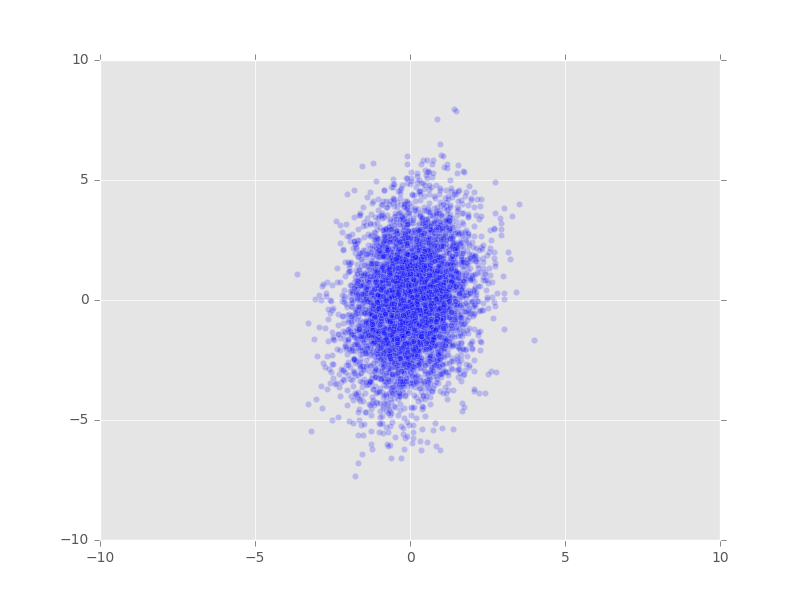
\includegraphics[width=450px]{/images/ppca-fig0.png}

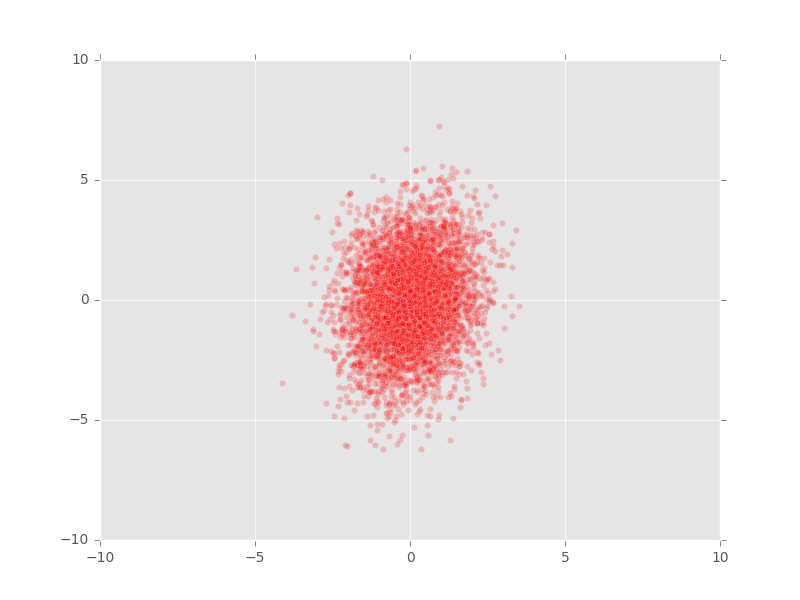
\includegraphics[width=450px]{/images/ppca-fig1.png}

\subsubsection{References}\label{references}
